\subsection{Model comparison and feature attribution}
\label{sec:result-model_comp}


The trained \emph{Ridge}, \emph{XGBoost}, and \emph{DE} models with structures and training details in Sect.~\ref{sec:methods-models,sec:method-daataset-split} are compared for their performance over withheld test data and corrected real OCO-2 data. We use ocean and land footprints from the training set to train separate models for ocean and land for all structures. Each model has $5$ members, which are trained on different folds of data (Fig.~\ref{fig:5fold_illustration}). Table~\ref{tab:cv-model-comparison} shows the performance of three models on the same held-out test data. The \emph{DE} has the lowest $RMSE$ and highest $R^2$ when comparing the predicted and true $\Delta$\xcobc, which is better than the \emph{XGBoost} and \emph{Ridge} baselines.


In addition to the $5$ folds held-out test data, we also compare their performance on corrected \xco, which is calculated by
%
\begin{equation}
  \mathrm{X_{CO2}^{model}} = \mathrm{X_{CO2}^{B11}} - \Delta \mathrm{X_{CO2}^{predicted}},
  \label{eq:xco2_corr}
\end{equation}
%
which $\Delta \mathrm{X_{CO2}^{predicted}}$ is predicted \xco anomaly, and $\mathrm{X_{CO2}^{model}}$ is the corrected \xco from different models. The \xcobc, $\mathrm{X_{CO2}^{Ridge}}$, $\mathrm{X_{CO2}^{XGBoost}}$, and $\mathrm{X_{CO2}^{DE}}$ are compared with TCCON measurements following the evaluation method described in Sect.~{sec:method-eval}. Similar to the results of $5$ folds held-out test data, the \emph{DE} model leads at every slice, and the model performance difference is larger in the near-cloud land tail (Fig.~\ref{fig:model_baseline_ablation}a). Though the difference is smaller in the near-cloud ocean tail, the \emph{DE} model still performs better if we consider both the near-cloud ocean tail and QF1 footprints. 

The same ordering holds on the withheld date-blocked folds of the anomaly target (Appendix~\ref{app:model_compare}, Fig.~\ref{fig:model_cv_compare}). The agreement between internal held-out and the independent validations means neither the target construction nor the TCCON chain is driving the selection. Though the fold metrics understate the gap, since the \emph{XGBOOSt} model trails the \emph{DE} model by only ~0.02–0.04 ppm in fold RMSE but by 0.25 ppm on the near-cloud land (≤15 km) TCCON tail. As a result, the \emph{DE} model is used in the later analysis.


After testing the performance over withheld test data and corrected real OCO-2 data, we are interested in the contribution of the feature groups and individual features. We first test removing (1) retrieval-state feature (\xcoraw − \xcoprior), (2) spectral path-length features, and (3) contamination features (See detailed features in Table~\ref{tab:training-config}). As shown in Fig.~\ref{fig:model_baseline_ablation}b, dropping the spectral or contamination groups is TCCON-neutral, whereas removing the retrieval-state departure \xcoraw − \xcoprior) costs 0.8–1.2 ppm. Although using "\xcoraw − \xcoprior" as a feature is similar to looking for an answer of $\Delta$ \xcobc, the $R^2$ between "\xcoraw − \xcoprior" and $\Delta$ \xcobc is only 0.323 for ocean and 0.191 for land. In other words, "\xcoraw − \xcoprior" carries the most abundant cloud-induced \xco bias information, but does not directly reflect the $\Delta$ \xcobc. Even "\xcoraw − \xcoprior" is the most important feature compared to spectral path-length and contamination feature groups, dropping "\xcoraw − \xcoprior" with either spectral path-length or contamination feature groups can degrade the $\Delta \mathrm{RMSE}$ more than not using "\xcoraw − \xcoprior" itself. In particular, dropping "\xcoraw − \xcoprior" with spectral-fitting features shows the largest $\Delta \mathrm{RMSE}$ increase for pooled, near-cloud land and near-cloud ocean tests.


Although the spectral path-length group seems to contribute less than "\xcoraw − \xcoprior" alone, its value lies in three roles "\xcoraw − \xcoprior" cannot fill. First, it indicates the mechanism of cloud-induced bias. The sign rule and shadow/brightening branches of Sect.~\ref{sec:result-spec_anal} establish that the corrected signal is a photon path-length effect, which is something the retrieval-state channel exploits but cannot demonstrate. Second, the spectral path-length group increases the safety of over-correction. The band-resolved fingerprint of Sect.~\ref{sec:result-plume} bounds what the correction may remove. The channel attribution shows the full model removes 55 \% (40–63 \%) of plume-free local clear-sky spread, the no-spectral variant removes 54 \% (the cumulants contribute none of the smoothing essentially), and the no-retrieval-state variant removes 29 \%. The local smoothing flows through the retrieval-state channel while the spectral channel supplies the plume-versus-cloud discriminator. Third, this feature group provides the robustness of imager-independent correction. The cloud-proximity sensitivity of the spectra, including below the MODIS resolution floor (Supplement S4), is what makes imager-free deployment and cross-sensor transfer (Sect.~\ref{sec:disc-img-free}, Appendix H) conceivable. In short, the spectral path-length features establish what the bias is and bound what the correction may touch, while the retrieval-state feature is the operationally sufficient predictor of it.






\begin{figure}[t]
\centering
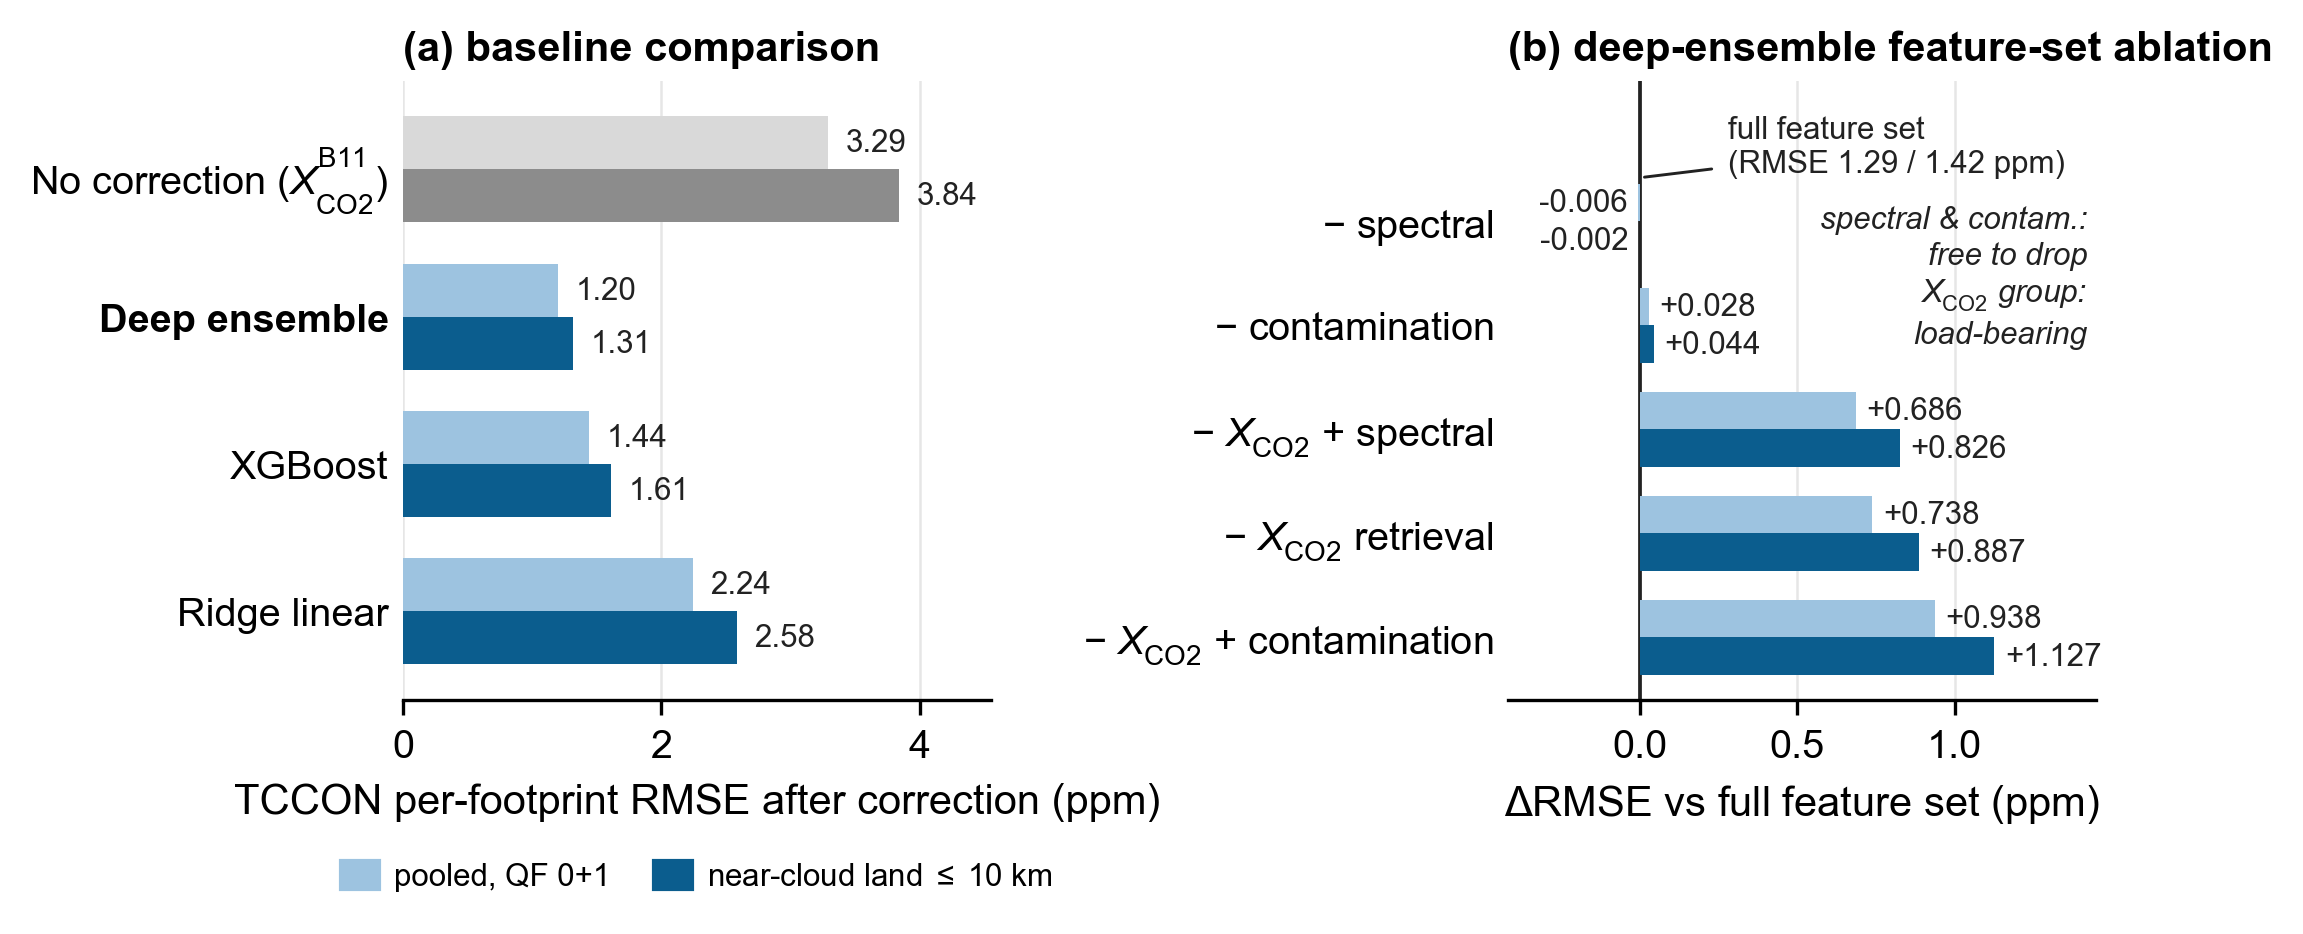
\includegraphics[width=0.8\textwidth]{figures/fig06_baseline_ablation.png}
\caption{Model and feature-set comparison under one protocol (identical features, date-blocked folds, and TCCON chain; AK-harmonised, r = 100 km / ±60 min). (a) TCCON per-footprint RMSE after correction, pooled over all quality flags (light, n = 105,683) and for the near-cloud land subset (≤ 10 km, dark, n = 75,157); the uncorrected product is shown for reference. (b) Feature-group ablation of the deep ensemble: $\Delta$RMSE relative to the full feature set.}
\label{fig:model_baseline_ablation}
\end{figure}



We then evaluate the permutation importance of each variable in the predictors by randomly shuffling each variable to see the increase in $\Delta \mathrm{RMSE}$ for the \emph{DE} model. Same as the results in Fig.~\ref{fig:model_baseline_ablation}b, the "\xcoraw − \xcoprior" plays the most essential role in the bias prediction for both the ocean and land models. The "$\Delta \mathrm{P}$/$\mathrm{P_{surface}^{prior}}$" shows as the second most important variable for both surfaces. Among the spectral path-length features, "var($l'$) of W\ce{CO2}" has the strongest response for the ocean model and the second strongest for the land model. The "$\exp$(\ce{O2}A intercept)" is the most important spectral path-length feature for the land model. The PC1 and PC2 of \ce{CO2} profile EOFs are also crucial for the prediction. Since cloud-bias information can be distributed across several variables in different ways, permuting individual variables may not capture the true importance of each feature. However, this analysis still helps us understand the potential importance of the features.




\begin{figure}[t]
\centering
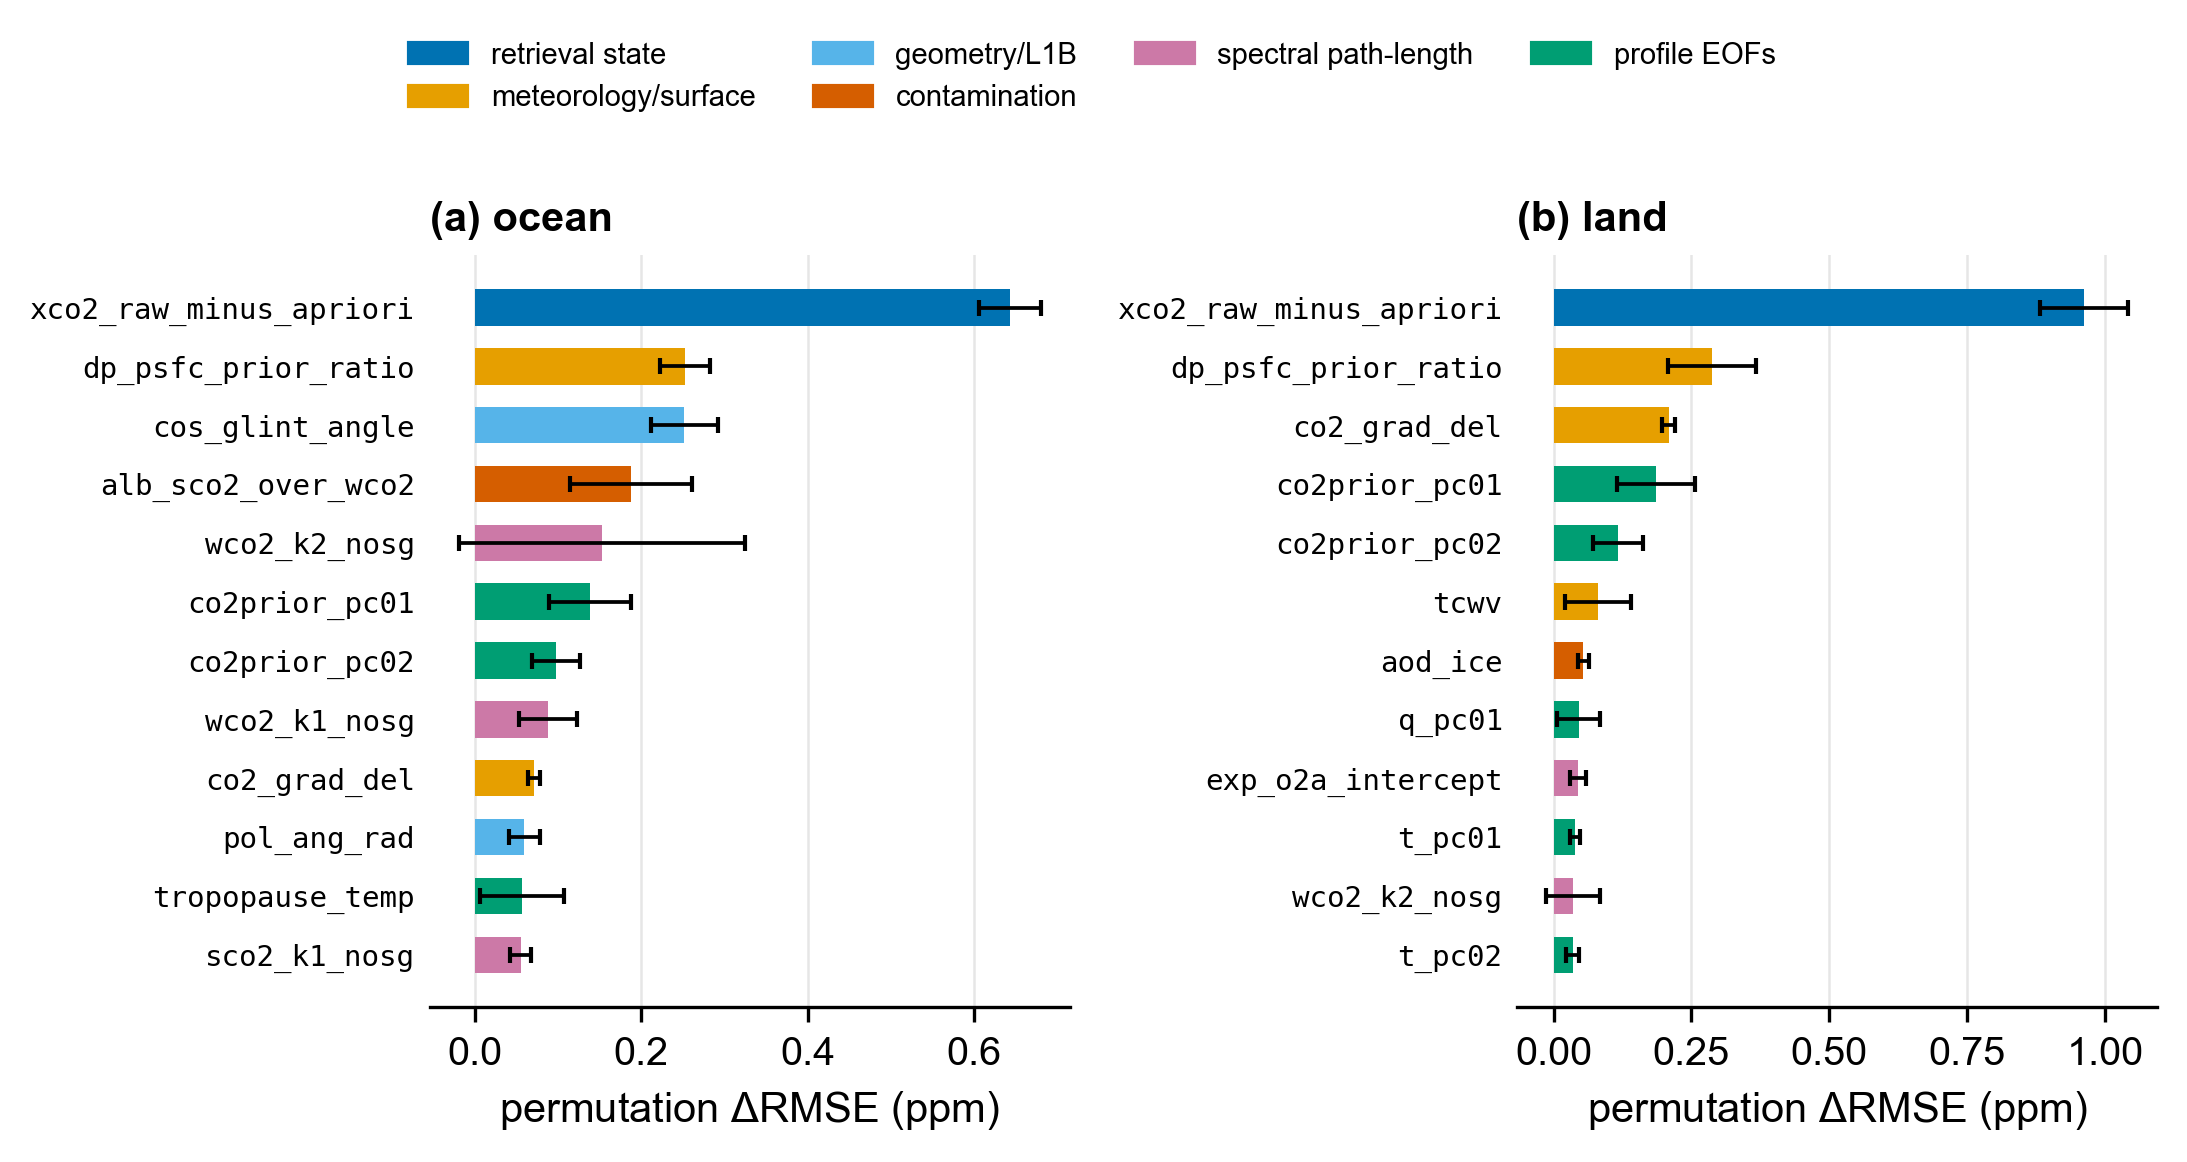
\includegraphics[width=0.8\textwidth]{figures/fig07_feature_importance.png}
\caption{Per-feature permutation importance of the production deep ensemble: increase in held-out fold RMSE when one feature is permuted (median over the five date-blocked folds; whiskers, fold standard deviation), for the twelve highest-ranked features over (a) ocean and (b) land. Bar color gives the predictor group of each feature, with feature definitions in Table~\ref{tab:predictor-inventory}. Groups are permuted jointly in the group-level attribution (Fig.~\ref{fig:model_baseline_ablation}b), which is the appropriate quantity under feature collinearity.}
\label{fig:DE_feature_importance}
\end{figure}




% Generated by manuscript/scripts/make_manuscript_tables.py — do not hand-edit.
% Requires booktabs. Define in the preamble:
%   \newcommand{\xcobc}{$X_{\mathrm{CO2}}^{\mathrm{bc}}$}
%   \newcommand{\xcoraw}{$X_{\mathrm{CO2}}^{\mathrm{raw}}$}
\begin{table}[htbp]
\centering
\caption{Footprint RMSE against AK-harmonized TCCON (ppm; 100\,km / $\pm$60\,min, 75 station-days) before (\xcobc) and after correction by the deep ensemble (DE), XGBoost (XGB), and ridge regression (Ridge). All models share the same footprints and before-column; the best corrected value per slice is in bold. QF is the operational \texttt{xco2\_quality\_flag}; cloud-distance slices split each surface at its production target radius (ocean 5\,km, land 15\,km; Sect.~3.1) and use the pre-drift cases where the Aqua-MODIS collocation is reliable.}
\label{tab:model-comparison}
\small
\begin{tabular}{lrrrrr}
\specialrule{1.2pt}{0pt}{2pt}
Slice & $n$ & Before & DE & XGB & Ridge \\
\midrule
Pooled, QF 0+1 & 105\,683 & 3.29 & \textbf{1.22} & 1.43 & 2.27 \\
Pooled, QF$\,$=$\,$0 & 56\,085 & 1.01 & \textbf{0.83} & 0.87 & 0.92 \\
Pooled, QF$\,$=$\,$1 & 49\,598 & 4.68 & \textbf{1.54} & 1.88 & 3.16 \\
Ocean & 6\,249 & 1.27 & \textbf{0.98} & 1.11 & 1.16 \\
Ocean, QF$\,$=$\,$1 & 1\,578 & 1.76 & \textbf{1.25} & 1.47 & 1.56 \\
Ocean $\leq$5\,km & 2\,645 & 1.54 & \textbf{1.12} & 1.24 & 1.26 \\
Ocean $\leq$5\,km, QF$\,$=$\,$1 & 1\,080 & 1.92 & \textbf{1.29} & 1.46 & 1.52 \\
Ocean $\geq$5\,km & 3\,604 & 1.02 & \textbf{0.86} & 1.01 & 1.08 \\
Land & 99\,434 & 3.38 & \textbf{1.23} & 1.45 & 2.32 \\
Land, QF$\,$=$\,$1 & 48\,020 & 4.75 & \textbf{1.55} & 1.89 & 3.20 \\
Land $\leq$15\,km & 81\,347 & 3.71 & \textbf{1.31} & 1.56 & 2.52 \\
Land $\leq$15\,km, QF$\,$=$\,$1 & 44\,107 & 4.94 & \textbf{1.59} & 1.94 & 3.32 \\
Land $\geq$15\,km & 18\,087 & 0.95 & \textbf{0.79} & 0.85 & 0.98 \\
\specialrule{1.2pt}{2pt}{0pt}
\end{tabular}
\end{table}






% Generated by manuscript/scripts/make_manuscript_tables.py — do not hand-edit.
% Requires booktabs. Define in the preamble:
%   \newcommand{\xcobc}{$X_{\mathrm{CO2}}^{\mathrm{bc}}$}
%   \newcommand{\xcoraw}{$X_{\mathrm{CO2}}^{\mathrm{raw}}$}
\begin{table}[htbp]
\centering
\caption{Feature-group ablation of the mix deep ensemble on TCCON (fp-RMSE, ppm; AK-harmonized reference, 100\,km / $\pm$60\,min). Each variant is retrained from scratch with one feature group removed, using the identical architecture, regularization, and date-blocked folds as the production model (full); all columns share the same footprints and before-column. Dropping the spectral-cumulant or aerosol-contamination groups is TCCON-neutral; the \xcoraw$-$prior departure block carries the correction.}
\label{tab:featureset-ablation}
\small
\begin{tabular}{lrrrrrrr}
\specialrule{1.2pt}{0pt}{2pt}
Slice & Before & full & $-$spec & $-$contam & $-$xco2 & $-$xco2$-$spec & $-$xco2$-$contam \\
\midrule
Pooled, QF 0+1 & 3.29 & \textbf{1.22} & 1.24 & 1.24 & 2.01 & 2.15 & 2.11 \\
Pooled, QF$\,$=$\,$0 & 1.01 & 0.83 & \textbf{0.83} & 0.85 & 1.03 & 0.99 & 1.12 \\
Pooled, QF$\,$=$\,$1 & 4.68 & \textbf{1.54} & 1.58 & 1.58 & 2.72 & 2.96 & 2.84 \\
Ocean & 1.27 & \textbf{0.98} & 1.00 & 0.99 & 1.13 & 1.15 & 1.15 \\
Land & 3.38 & \textbf{1.23} & 1.25 & 1.26 & 2.05 & 2.20 & 2.16 \\
Land, QF$\,$=$\,$1 & 4.75 & \textbf{1.55} & 1.59 & 1.59 & 2.76 & 2.99 & 2.88 \\
Land $\leq$10\,km & 3.84 & \textbf{1.33} & 1.36 & 1.36 & 2.30 & 2.47 & 2.42 \\
Land $\leq$10\,km, QF$\,$=$\,$1 & 5.00 & \textbf{1.60} & 1.64 & 1.63 & 2.88 & 3.14 & 3.01 \\
Land $\geq$10\,km & 1.00 & 0.84 & \textbf{0.83} & 0.90 & 0.91 & 0.97 & 0.98 \\
\specialrule{1.2pt}{2pt}{0pt}
\end{tabular}
\end{table}






\FloatBarrier